\begin{center}
    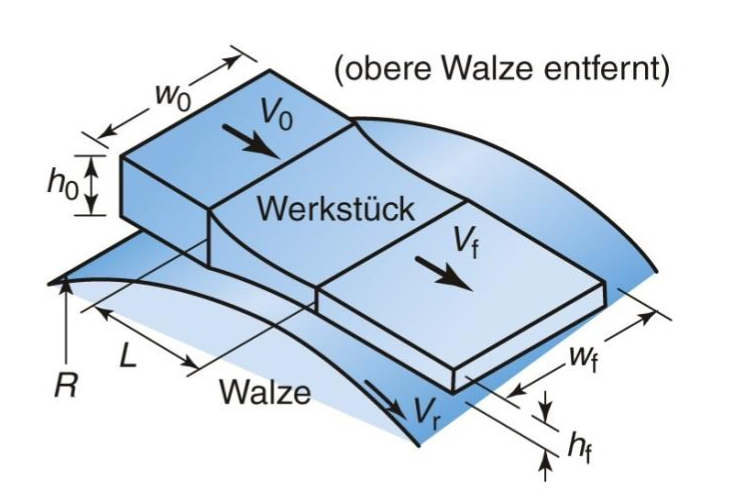
\includegraphics[width = 40mm]{src/images/Walzen.png}\\
\end{center}
\textbf{Ziel:}\\
$\downarrow$ Dicke, $\downarrow$ Fehler aus dem Giessprozess, Einstellen mechanischer Eigenschaften (Festigkeit, Textur).\\

\textbf{Warmwalzen:}\\
$\downarrow$ der Korngrösse, $\uparrow $ mechanischen Eigenschaften. \\
Warmwalzen erzeugt eine schlechtere Oberfläche als Kaltwalzen.\\
\vfill \null \columnbreak

\textbf{Durchbiegung:}\\
Führt zu Ausbauchung im Werkstoff.\\
Gegenmassnahmen: 
Stützwalzen, Vorspannung oder konvexe Walzen\\
